我们在初中和高中的学习中学习了很多的``关系''. 比如, 比较两个数的大小, 我们引入了``大于'', ``小于''和``等于''的关系. 这样的内容我们可以进一步的抽象, 提炼出``关系''的一些共性. 

比如, 我们可以在$\R$上定义``Near''关系.

\begin{eg}
    如果$|a - b| < 1(a, b \in \R)$, 则称$a, b$具有Near关系. 
\end{eg}

回顾我们学过的表达``关系''的运算符, 相当一部分满足下面的性质: 

\textbf{自反性. }
$$\forall a \in X.\; (a, a) \in R$$

\textbf{对称性. }
$$\forall a, b \in X.\; ((a, b) \in R \to (b, a) \in R)$$

\textbf{传递性. }
$$\forall a, b, c \in X.\; ((a, b) \in R \land (b, c) \in R \to (a, c) \in R)$$

很多时候, 自反性 + 对称性 = 相容关系. 相容关系的含义其实是表明这两个关系之间有交叉.\footnote{不是很确定直观上表示什么. } 

这样, 我们就可以把关系表示成一个集合. 不严格的说, 在上面的定义中, 我们可以有这样的集合: $R = \set{(a, b) \mid |a - b| < 1}$. 

下面来看几个更多的例子. 比如整除关系. 

\begin{eg}
    假设$X = \set{1, 2, 3, 4, 5, 6, 10, 12, 15, 20, 30, 60}$, ``关系''是$X$ 上的整除关系. 
\end{eg}

按照上面的展开, 我们就有所有整除的全体(有序对$(a,b)$表示的关系是$a|b$):
$$R = \set{(1, 2), \dots, (4, 12), \dots, (12, 60), \dots, (4, 60), \dots, (60, 60)}$$

可以看到在上述的关系中, 上面的自反性, 对称性, 传递性仍然满足. 这种结构十分的常见. 比如地图上面的地方的``可达''关系, 还有给定集合的幂集按``包含''关系排序, 自然数按照大小关系排序, 等等. 满足上述的三条性质的关系叫做``偏序关系''. 特殊的, 我们或许还会发现自然数可以唯一地按照大小被排成一排, 这是一种比较特殊的偏序关系, 后来我们会定义它为全序关系. 

特别的, 我们可以把上述偏序关系画成一张图, 也就是在多个维度上都有不同的序, 因此没办法唯一的列成一列, 包含所有元素. 

比如上述的幂集的例子, 化作一张图如下图所示: 
\begin{center}
    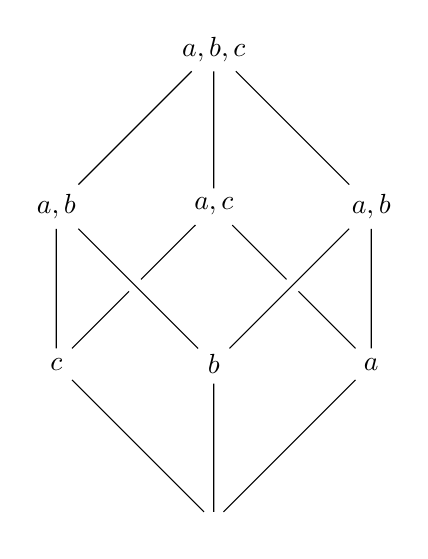
\begin{tikzpicture}
    \node (max) at (0,4) {$\set{a,b,c}$};
    \node (a) at (-2,2) {$\set{a,b}$};
    \node (b) at (0,2) {$\set{a,c}$};
    \node (c) at (2,2) {$\set{a,b}$};
    \node (d) at (-2,0) {$\set{c}$};
    \node (e) at (0,0) {$\set{b}$};
    \node (f) at (2,0) {$\set{a}$};
    \node (min) at (0,-2) {$\set{}$};
    \draw (min) -- (d) -- (a) -- (max) -- (b) -- (f)
    (e) -- (min) -- (f) -- (c) -- (max)
    (d) -- (b);
    \draw[preaction={draw=white, -,line width=6pt}] (a) -- (e) -- (c);
  \end{tikzpicture}
\end{center}

观察正整数集, 发现这是一条链式结构, 它和上述的偏序集最大的区别是什么呢? 其实, 最大的区别是在整数中的大于关系存在``连接性''. 

\textbf{连接性.} 
$$
\forall a, b \in X.\; ((a, b) \in R \lor (b, a) \in R)
$$

也就是自反性 + 反对称性 + 传递性 + 连接性 = \red{\bf 全序关系}. 

\subsection{有序对}

我们可能会很自然的想$ (a, b) = (c, d) \iff a = c \land b = d$, 对于这样自然产生的概念, 我们同样要将它严格化, 给出一个定义.  

历史上, 很多人会用集合的观念来刻画有序对. Norbert Wiener在1914年给出了这样的定义. 

\begin{definition}[Ordered Pairs \teal{(Norbert Wiener; 1914)}]
    \[
      (a, b) \;\red{\triangleq}\; \Bset{\bset{\set{a}, \emptyset}, \bset{\set{b}}}
    \]
\end{definition}

这样一来, 有序对之间的相等关系看上去就自然了很多. 

\begin{theorem}
    \[
      (a, b) = (c, d) \iff a = c \land b = d
    \]
\end{theorem}
\begin{proof}
    也就是证明
    $$\Big(\bset{\set{a}, \set{a, b}} = \bset{\set{c}, \set{c, d}}\Big) \iff (a = c \land b = d)$$
    我们有: 
    \begin{align*}
        &\bset{\set{a}, \set{a, b}} = \bset{\set{c}, \set{c, d}} \\
        \iff& (\set{a} = \set{c} \lor \set{a} = \set{c, d}) \land (\set{a, b} = \set{c} \lor \set{a, b} = \set{c, d}) \\
        \iff& (\set{a} = \set{c} \land \set{a, b} = \set{c}) \;\lor \\
                         & (\set{a} = \set{c} \land \set{a, b} = \set{c, d}) \;\lor \\
                         & (\set{a} = \set{c, d} \land \set{a, b} = \set{c}) \;\lor \\
                         & (\set{a} = \set{c, d} \land \set{a, b} = \set{c, d})
      \end{align*}
    

\end{proof}

有了有序对, 我们还可以把它拓广到$n$个元素的情况. 于是我们有定义: 

\begin{definition}[$n$-元组 (n-ary tuples)]
    \[
      (x, y, z) \triangleq ((x, y), z)
    \]
    \[
      (x_{1}, x_{2}, \dots, x_{n-1}, x_{n})
        \triangleq ((x_{1}, x_{2}, \dots, x_{n-1}), x_{n})
    \]
\end{definition}

在这个结构上同样是可以应用数学归纳法的. 不过一般我处理而二元组就行了. 多数情况下, 我们仅处理``二元关系'', 因此也仅使用``有序对''

\subsection{笛卡尔积: 一种组合方式}

如果我们有两个集合, 从两个集合中各取得一个元素, 把它们组合成一个有序对,塞到一个新的集合里面, 这样, 我们就可以对于集合做一点组合, 生成更加复杂的集合了. 这样的操作叫做笛卡尔积.  

\begin{definition}[笛卡尔积 (Cartesian Products)]
    The \red{\it Cartesian product} $A \times B$ \blue{of $A$ and $B$}
    is defined as
    \[
      {A \times B \triangleq \set{(a, b) \mid a \in A \land b \in B}}
    \]
\end{definition}

那么``笛卡尔积''这个操作满足哪些运算律呢? 我们首先来考察一些例子. 

\begin{eg}
  
  \begin{align*}
  X\times \emptyset = \emptyset \times X \\
  X\times Y \neq  Y \times X \\
  (X \times Y) \times Z \;\neq\; X \times (Y \times Z)\\
  A = \set{1} \qquad (A \times A) \times A \;\red{\neq}\; A \times (A \times A)
  \end{align*}
  
\end{eg}

我们发现这个符号既没有普遍的交换律, 也没有普遍的结合律. 但是是有分配律的. 

\begin{theorem}[分配律 (Distributivity)]
  \[
    A \times (B \cap C) = (A \times B) \cap (A \times C)
  \]
  \[
    A \times (B \cup C) = (A \times B) \cup (A \times C)
  \]
  \[
    A \times (B \setminus C) = (A \times B) \setminus (A \times C)
  \]
\end{theorem}

下面我们来以证明$A \times (B \cap C) = (A \times B) \cap (A \times C)$为例, 看一下这个是如何进行起作用的. 
\begin{proof}
  \red{对任意\blue{有序对} $(a, b)$,}
    \setcounter{equation}{0}
    \begin{align}
      &(a, b) \in A \times (B \cap C) \\
      \iff& a \in A \land b \in (B \cap C) \\
      \iff& a \in A \land b \in B \land b \in C \\
      \iff& (\blue{a \in A} \land b \in B) \land (\blue{a \in A} \land b \in C) \\
      \iff& (a, b) \in A \times B \land (a, b) \in A \times C \\
      \iff& (a, b) \in (A \times B) \cap (A \times C)
  \end{align}
\end{proof}

同样的, 我们可以有多个元素的笛卡尔积. 

\begin{definition}[$n$-元笛卡尔积 ($n$-ary Cartesian Product)]
  \[
    X_{1} \times X_{2} \times X_{3} \triangleq (X_{1} \times X_{2}) \times X_{3}
  \]
  \[
    X_{1} \times X_{2} \times \dots \times X_{n}
      \triangleq (X_{1} \times X_{2} \times \dots \times X_{n-1}) \times X_{n}
  \]
\end{definition}

回想我们从数轴到平面直角坐标系再到空间直角坐标系, 我们可以发现这样的过程也就是对于一个维度反复做笛卡尔积的结果. 

但在本节的情况下, 我们仅处理``二元关系'', 因此也仅使用``二元笛卡尔积''. 


\subsection{用有序对定义二元关系}

我们以前做了有关关系的定义, 但是我们可能还要给``什么是关系''在集合方面下一个稍微集合化的定义. 于是我们有定义: 
\begin{definition}[关系 (Relations)]
  A \red{\it relation} $R$ \blue{from $A$ to $B$}
  is a \teal{subset} of $A \times B$:
  \[
    {R \subseteq A \times B}
  \]
  Sepcially, if $A = B$, $R$ is called a relation \blue{on} $A$.
\end{definition}

为了简化符号, 我们有时候也通过这样的方式来书写: 

\begin{definition}[Notations]
  \[
    (a, b) \in R \qquad a R b
  \]
  \[
    (a, b) \notin R \qquad a \overline{R} b
  \]
\end{definition}

举一些例子: $A\times B$ 和 $\emptyset$ 都是从 $A$ 到 $B$ 的关系, 前者的意义是任意两个$A$和$B$中的元素都有关系, 后者是都没有关系. 回顾我们在小学中学更一般的关系, 我们就会发现有更加有趣的二元关系: 
\begin{itemize}
  \item 小于关系: $<\; = \set{(a, b) \in \mathbb{R} \times \mathbb{R} \mid a \text{ is less than } b}$
  \item 整除关系: $D = \set{(a, b) \in \mathbb{N} \times \mathbb{N} \mid \exists q \in \mathbb{N}.\; a \cdot q = b}$
\end{itemize}

在生活中更有这样的关系. 比如$P$是所有人的集合, 如果我们定义$\red{M} = \set{(a, b) \in P \times P \mid a \text{ is the mother of } b}$, $\red{B} = \set{(a, b) \in P \times P \mid a \text{ is the brother of } b}$, 那么上述定义的$M$和$B$都满足``关系''的定义.

有了这样的抽象, 我们就可以很开心的研究另外一些更重要的问题了. 具体地, 我们要研究这些重要的关系: 
\begin{itemize}
  \item 等价关系
  \item 序关系
  \item 函数
\end{itemize}



